% Nallino, Part II p. 246, first figure: the first station on the epicycle, redrawn from the print at the size of the
% print. The coordinates are those of a 400 dpi render of the figure (crop from x 118 pt, y 190 pt of the master
% page; y downward). The epicycle has its centre in H; P and D are its true apogee and perigee on the line from the
% Earth E; the line EK cuts the epicycle in T and K, L the foot of the perpendicular from H; HL and HT are dotted.
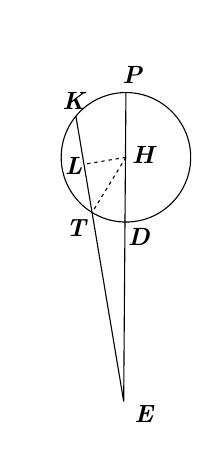
\begin{tikzpicture}[x=0.0635mm,y=-0.0635mm,line width=0.4pt,every node/.style={font=\bfseries\itshape\small,inner sep=1pt}]
\path (0,7.8);
\coordinate (H) at (196.5,267);
\coordinate (E) at (192,755);
\coordinate (K) at (96.5,185);
\coordinate (T) at (128.7,377.5);
\coordinate (L) at (112.6,281.1);
\draw (H) circle[radius=129.5];
\draw (196.5,137.5) -- (E);
\draw (K) -- (E);
\begin{scope}[dash pattern=on 1.2pt off 1.4pt]
\draw (H) -- (L);
\draw (H) -- (T);
\end{scope}
\node at (209,102) {P};
\node at (91.5,154) {K};
\node at (230.5,261.5) {H};
\node at (92,285) {L};
\node at (96.5,407.5) {T};
\node at (222,426.5) {D};
\node at (232,781) {E};
\end{tikzpicture}
